\documentclass[11pt, a4paper]{article}
\usepackage[utf8]{inputenc}
\usepackage[T1]{fontenc}
\usepackage{helvet}
\renewcommand{\familydefault}{\sfdefault}
\usepackage[table]{xcolor}
\definecolor{schoolgreen}{HTML}{92D050}
\usepackage{geometry}
\geometry{landscape, margin=2cm, top=4cm, headheight=2.5cm, headsep=0.5cm}
\usepackage{array}
\usepackage{longtable}
\usepackage{graphicx}
\usepackage{fancyhdr}

\pagestyle{fancy}
\fancyhf{}
\fancyhead[L]{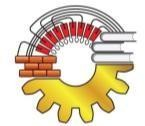
\includegraphics[height=2cm]{../../distritos/4117/templates/logo1.jpg}}
\fancyhead[R]{
\includegraphics[height=2cm]{../../distritos/4117/templates/logo2.jpg}}
\fancyhead[C]{\fontsize{10}{12}\selectfont \textbf{\textit{ESCUELA N.° 4-117 EJÉRCITO DE LOS ANDES \\ DIRECCIÓN DE EDUCACIÓN TÉCNICA Y TRABAJO \\ SECCIÓN V}}}
\renewcommand{\headrulewidth}{0pt}

\begin{document}

\noindent\colorbox{schoolgreen}{\begin{minipage}{\dimexpr\textwidth-2\fboxsep}\centering \textbf{\fontsize{14}{16}\selectfont PROGRAMA 2026}\end{minipage}}

\vspace{1em}

\begin{flushleft}
\textbf{Espacio Curricular:} Prácticas Profesionalizantes \\
\textbf{Ciclo Lectivo:} 2026 \\
\textbf{Curso:} 5to 3ra \\
\textbf{Profesor/a Responsable:} Ferreyra Gustavo David
\end{flushleft}

\vspace{1em}

\begin{longtable}{|p{\dimexpr\textwidth-2\tabcolsep-2\arrayrulewidth}|}
\hline
\rowcolor{gray!20} \textbf{Contenidos Programáticos} \\
\hline
\textbf{EJE Nº 1: MARCO NORMATIVO, SEGURIDAD Y ÉTICA PROFESIONAL} \\
$\bullet$ Normas de Seguridad e Higiene, EPP y Señalética Industrial. \\
$\bullet$ Marco Jurídico aplicado a la actividad técnica y profesional. \\
$\bullet$ Acuerdos de convivencia y ética en el entorno laboral. \\
$\bullet$ Gestión de riesgos y protocolos de prevención de accidentes. \\
\hline
\textbf{EJE Nº 2: PLANIFICACIÓN Y GESTIÓN DE PROYECTOS TÉCNICOS} \\
$\bullet$ Metodologías de organización: Diagramas de Gantt y Tableros Kanban. \\
$\bullet$ Estudio de tiempos y movimientos en procesos productivos. \\
$\bullet$ Elaboración de anteproyectos electromecánicos y diseño de instalaciones. \\
$\bullet$ Gestión de la idea y formulación de proyectos técnicos. \\
\hline
\textbf{EJE Nº 3: ANÁLISIS ECONÓMICO Y EMPRENDIMIENTO} \\
$\bullet$ Estructura de costos: Costos fijos, variables y punto de equilibrio. \\
$\bullet$ Estudio de mercado, definición de alcances y valor económico de servicios. \\
$\bullet$ Comercialización y asesoramiento en máquinas e instalaciones electromecánicas. \\
$\bullet$ Evaluación de viabilidad económica de microemprendimientos técnicos. \\
\hline
\textbf{EJE Nº 4: EJECUCIÓN TÉCNICA, CALIDAD Y REFLEXIÓN} \\
$\bullet$ Ejecución de montaje, reparaciones y mantenimiento industrial. \\
$\bullet$ Operación de máquinas-herramientas y control de calidad de procesos. \\
$\bullet$ Diagramas de flujo de procesos y optimización de tareas. \\
$\bullet$ Elaboración de informes técnicos y reflexión crítica del desempeño profesional. \\
\hline
\end{longtable}

\end{document}